\section{Reducing preparation around the learned choices}
\label{sec:parametric}
The previous comparison leaves a substantial cost even after the model has chosen a useful seed region. On a four-loop development batch, the actual row operations take a small fraction of the total time, while sector symmetry preparation and repeated equation generation dominate. We therefore retain the trained policies and change the exact work that surrounds their choices. This comparison tests whether better integration can make the same predictions more useful without adding another model or changing its weights.

\subsection{Avoiding unused polynomial terms and repeated equations}
Kira uses parametric polynomials to identify zero sectors and sector symmetries~\cite{KiraOriginal,Lee2014LiteRed}. Each inverse propagator has a Schwinger parameter, an auxiliary variable in this representation. An auxiliary inverse propagator can occur in a numerator while its index remains nonpositive throughout the declared sector domain. Its Schwinger parameter then vanishes in the sector polynomials used for these checks. The preceding implementation first constructs the full polynomials and removes the unused parameter terms from the zero-sector criterion. We now apply this substitution before polynomial construction and use the resulting restricted polynomials for both zero-sector and symmetry checks. Appendix~\ref{app:parametric} proves that this change gives the same polynomial in every admitted sector. The full propagator list remains available when Kira forms IBP identities and transforms numerators.

Kira also constructs selected symbolic equations to check their remaining masters, then constructs those equations again for the final reduction. We keep the unmodified exact rows from the first construction. When the next selection returns the identical ordered list of source equations, the calculation uses those saved rows. If the selection changes or the storage allowance is exceeded, Kira regenerates the equations normally. The saved rows exist only within that reduction; no previous target answer supplies a later result. This change removes a repeated calculation of an established identity. It does not replace equation selection or symbolic elimination.

The application uses the same trained portfolio, graph-specific predictors, thresholds, seed settings, worker choices, and recovery rules as Section~\ref{sec:portfolio}. We fit no model in this comparison. Thus any change relative to the previous application measures the exact integration changes and timing variation. A matched fixed-portfolio control measures the additional effect of the outer prediction. The earlier separate service remains available for the few requests assigned to it, and its full cost remains in the measurement.

\subsection{Fresh targets and matched controls}
We reserve 26 new batches from the same nine graph structures, with one to three targets per batch and loop orders one through four. The rational cases use a fresh parameter profile. The symbolic nonplanar and pentagon cases move the raised denominator power to a new position, while the virtuality box has two singly dotted denominators. Appendix~\ref{app:parametric} specifies these inputs. The frozen range guard can select native settings when a new target pattern lies outside its training range.

The first reference reduction uses expanded seeds with the revised preparation. A second calculation uses the previous executable and a larger numerator-rank limit to check the resulting coefficients in the same basis. Each timed method then receives the target and that prescribed basis. Reference coefficients enter only the comparison after the calculation. The test checks reduction to this basis, rather than proving that the basis is minimal.

We compare four methods: the previous application; native choices with revised preparation; a graph-specific fixed portfolio with revised preparation; and the selected portfolio with revised preparation. The fixed portfolio can contain an earlier learned policy, so it isolates the added outer choice. All methods use the same two-core allocation, memory limits, and exact checks. Native choices use one Kira worker, while the portfolios retain their chosen one or two workers. The revised controls share the application's input checks and portfolio proposal; the native and fixed controls then override that proposal. We report the effect of removing this common overhead below. Each attempt starts a fresh Kira process with fresh temporary files. Three repetitions rotate method order. Complete time includes decisions, input preparation, algebra, coefficient checks, cleanup, and unsuccessful attempts. Initial model loading, reference construction, and basis discovery remain outside these repeated timings.

\subsection{Results and attribution}
Table~\ref{tab:parametric} sums the median time of each batch. The revised selected application takes 64.183 seconds, compared with 79.784 seconds for the previous application. This is 19.6\% less time on the measured collection. The selected actions agree with the previous application for every batch and repetition, so this improvement comes from the exact preparation changes around the existing models. Summing all repetitions gives 19.6\% less time than the previous application.

\begin{table}[!htbp]\centering\small
\caption{Complete times in seconds, summed over batch medians. The previous column uses the earlier preparation. The other columns enable both exact changes for direct Kira attempts; the earlier separate service retains its preparation. Fixed denotes the validation-selected portfolio choice for each graph.}
\label{tab:parametric}
\begin{tabular}{@{}lrrrr@{}}\toprule
Graph & Previous & Native & Fixed & Selected\\\midrule
Sunrise (2 loops) & 1.742 & 1.706 & 1.806 & 1.793\\
Planar double box (2) & 6.155 & 8.501 & 7.123 & 5.953\\
Vacuum (3) & 2.788 & 2.678 & 2.678 & 2.636\\
Two-point ladder (3) & 13.393 & 23.400 & 12.917 & 11.581\\
Nonplanar box (2) & 19.794 & 28.662 & 20.478 & 20.052\\
Pentagon (1) & 3.094 & 2.989 & 3.003 & 3.022\\
Virtuality box (1) & 2.172 & 2.216 & 2.232 & 2.229\\
Bubble box (3) & 2.225 & 1.617 & 1.735 & 1.647\\
Bubble box (4) & 28.421 & 16.078 & 15.409 & 15.271\\
\midrule Total & 79.784 & 87.847 & 67.381 & 64.183\\\bottomrule
\end{tabular}\end{table}

With each candidate implemented in the same way for all controls, the selected method uses 26.9\% less time than native choices and 4.7\% less time than the fixed portfolio. Across all repetitions, its difference from the fixed portfolio is 5.0\% less time. These controls keep the effect of learned decisions separate from exact reuse. The graph results in Figure~\ref{fig:parametric} show the measured savings and regressions; a smaller total does not imply that every batch becomes faster.

The common interval for input checks and the outer proposal is at most 2.854 milliseconds per revised request. Removing this entire measured interval from the native and fixed controls gives optimistic totals of 87.828 and 67.363 seconds, respectively. The selected method then uses 4.7\% less time than this optimistic fixed control. This subtraction removes useful checks as well as the unused proposal and therefore serves as a sensitivity bound, rather than a separately timed implementation.

All 312 timed reductions and 26 further basis-only applications reproduce their checked reference coefficients exactly. The reference checks, timed tests, and applications compare 8,086 target--master coefficients. The revised selected method needs 6 recovery attempts across its timed tests. The recorded process-tree memory peak among the timed reductions is 961.8 MiB. The selected method takes 92.782 seconds in summed batch median CPU time, compared with 107.054 seconds for the previous application. The bounded replay mechanism activates 117 times across the timed controls and retains at most 0.221 MiB of accounted row data in an activation.

\begin{figure}[tbp]\centering
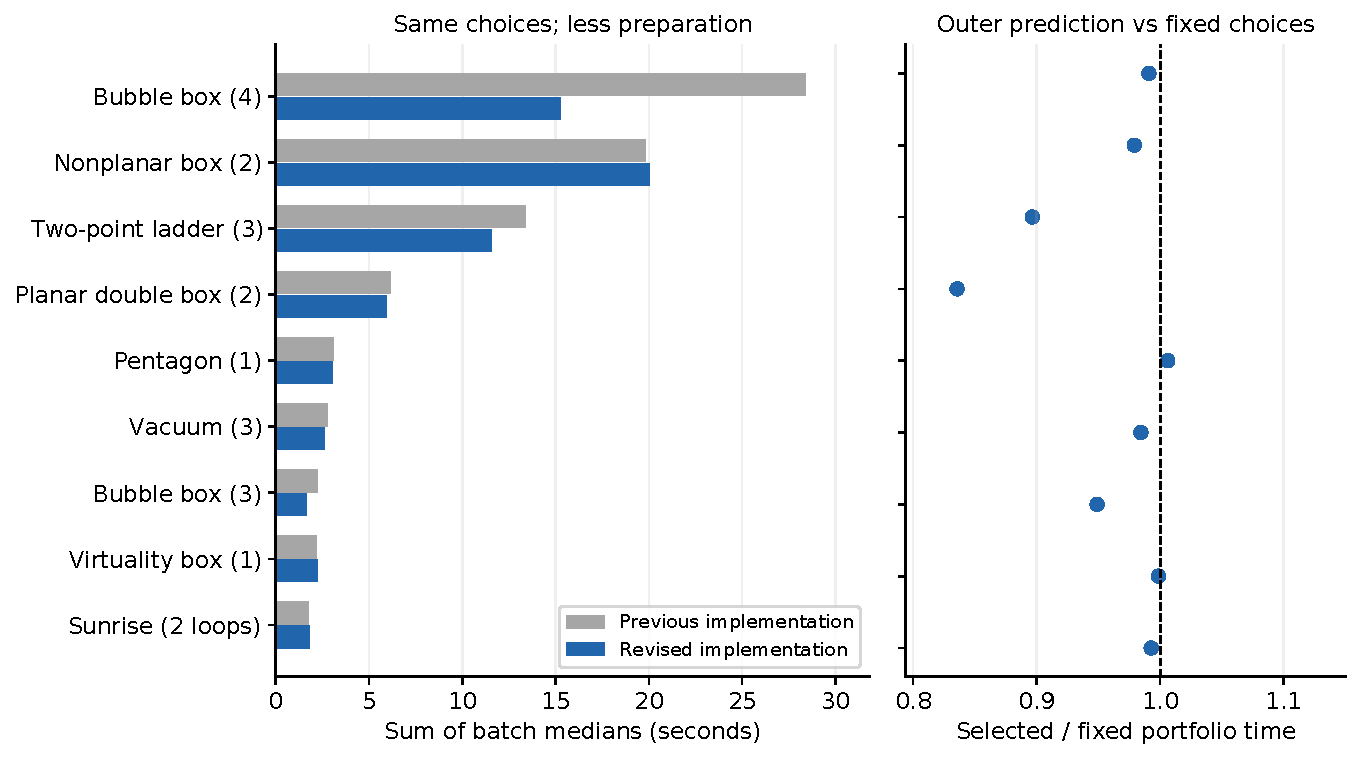
\includegraphics[width=\linewidth]{paper_figures/parametric_results.pdf}
\caption{Left: the same learned actions run with the previous and revised preparation. Right: the selected-to-fixed time ratio with revised preparation; the dashed line marks equal time. Each point or bar uses sums of batch medians within a graph. The right panel isolates the additional outer prediction.}
\label{fig:parametric}
\end{figure}

These results support the revised application for this measured collection. They test new parameters and target patterns within known graph structures, with supplied master bases. They do not establish general high-loop scattering performance or a globally shortest reduction. The earlier row-model result remains unchanged, so the application continues to use native row elimination.
